\section{Reactive\-Thread Class Reference}
\label{class_reactive_thread}\index{ReactiveThread@{ReactiveThread}}
Inheritance diagram for Reactive\-Thread::\begin{figure}[H]
\begin{center}
\leavevmode
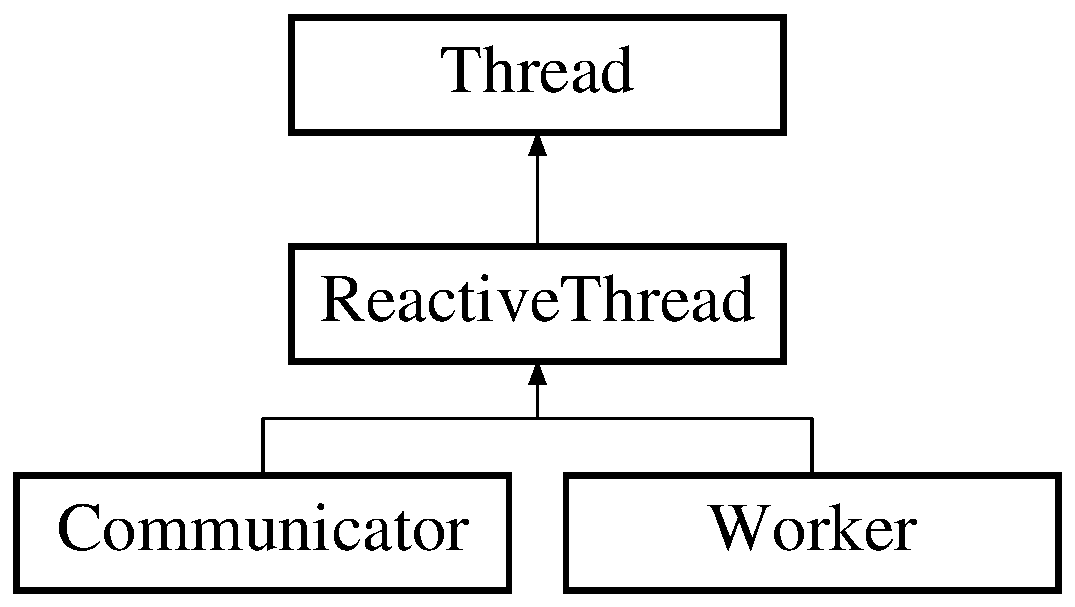
\includegraphics[height=3cm]{class_reactive_thread}
\end{center}
\end{figure}
\subsection*{Public Member Functions}
\begin{CompactItemize}
\item 
{\bf Reactive\-Thread} ()\label{class_reactive_thread_77381649429941c99a3e3d568113d6cf}

\item 
void {\bf sleep} ()\label{class_reactive_thread_8263c2a32d8c99a49a05f1a7717d4262}

\item 
void {\bf wake\-Up} ()\label{class_reactive_thread_a724a54575de10f09cc03ab7aa4e59ce}

\end{CompactItemize}
\subsection*{Private Attributes}
\begin{CompactItemize}
\item 
sem\_\-t {\bf sem}\label{class_reactive_thread_915e5a42dc8cb1bcf6738d5fe883a4e7}

\end{CompactItemize}


\subsection{Detailed Description}




Definition at line 31 of file reac\_\-thread.h.

The documentation for this class was generated from the following files:\begin{CompactItemize}
\item 
reac\_\-thread.h\item 
reac\_\-thread.cpp\end{CompactItemize}
